The rising of quantum computing in the last few years became the attention of researchers to schemes that uses cryptography primitives different from discrete logarithm and number factorization. As mentioned before in Chapter \ref{ch:intro}, code-based cryptosystems are those who use fundamental aspects of coding theory to add redundancy into a plain text, to after that, intentionally add some errors and recovery the plain text. 

In this chapter, we explain the first cryptosystem based on coding theory. Furthermore, we present a Round One code-based submission to the NIST standardization process, the BIGQUAKE, and we show the timing side-channel attack performed in the reference implementation of the scheme.

\section{McEliece Cryptosystem}
Robert J. McEliece proposes in 1978 the first cryptosystem based on coding theory, the McEliece cryptosystem was based on the Goppa codes and used them to achieve three main algorithms, i. e. Key Generation, Encryption and Decryption \cite{mceliece1978public}. Figure \ref{fig:code-idea} shows the main of the McEliece Cryptosystem and most of the schemes based on coding theory. Given a plaintext and a public encoding function, anyone can generate a codeword and intentionally add some errors to obtain a ciphertext. From this ciphertext, only who knows the code structure is able to perform a decoding function and recover the plaintext.


\begin{figure}
    \centering
    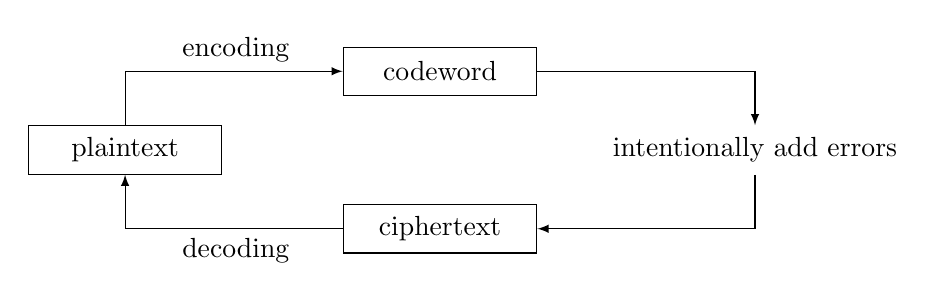
\begin{tikzpicture}
    \node[draw, minimum width=70pt, minimum height=17.5pt] (plain1) at (0, -1) {plaintext};
    \node[draw, minimum width=70pt, minimum height=17.5pt] (ciphertext) at (4, -2) {ciphertext};
    \node[draw, minimum width=70pt, minimum height=17.5pt] (codeword) at (4, 0) {codeword};
    \node[minimum width=70pt, minimum height=17.5pt] (adderror) at (8, -1) {intentionally add errors};
    \draw[-latex] (plain1) |- node[above, xshift=40pt]{encoding} (codeword);
    \draw[-latex] (codeword) -| (adderror);
    \draw[-latex] (adderror) |- (ciphertext);
    \draw[-latex] (ciphertext) -| node[below, xshift=40pt]{decoding} (plain1);
    \end{tikzpicture}
    \label{fig:code-idea}
    \fonte{the author.}
    \caption{Code-based cryptography main idea.}
\end{figure}

Based on two well know problems, the security of McEliece has remained stable. The first assumption was the hardness of generic decoding, and it is NP-complete and is also consider hard on average. The second assumption that regards the security of the McEliece scheme was the indistinguishability of the code. This second assumption is not as old as the first one, but it relates to old problems of algebraic coding theory and its consider valid for Goppa Codes, as the original proposal. 

The original parameters were designed for $2^{64}$ security bits, but it easily scales up to provide an ample security margin against attackers. Furthermore, the McEliece Cryptosystem suffers many structural attacks, and until today the original proposal is considered secure. It is important to note that many of these attacks based on the same strategy, the information set-decoding. This kind of attack does not affect schemes based on Goppa codes. However, many other families of codes suffer several drawbacks with this attack. 


As proposed in \cite{bernstein2017classic, bardet2017big} on the NIST standardization process, the McEliece cryptosystem, using binary Goppa codes, could be applied to concept a KEM, as defined in Chapter \ref{ch:math}. Based on this fact, we can generalize the cryptosystem in three algorithms: the Key generation and Encryption are defined in Section \ref{sub:mc-def} and Decryption in Section \ref{sub:mc-dec}.

\subsection{Definitions}
\label{sub:mc-def}
In this Section we describe the three main algorithms of the McEliece the McEliece cryptosystem based on irreducible binary Goppa code. 

Algorithm~\ref{alg:1} is the key generation of McEliece. First, it starts by generating a binary Goppa polynomial $g(z)$ of degree $t$, which can be an irreducible Goppa polynomial. Second, it generates the support $L$ as an ordered subset of $\mathbb{F}_{2^m}$ satisfying the root condition. Third, it is the computation of the systematic form of $\hat{H}$ is done using the Gauss-Jordan elimination algorithm. Steps four, five, and six compute the generator matrix from the previous systematic matrix and return secret and public key.

\begin{algorithm}[!ht]
 \KwData{$t, k, n, m$ as integers.}
 \KwResult{pk as public key, sk as secret key.}
 Select a random binary Goppa polynomial $g(z)$ of degree $t$ over $\mathbb{F}_{2^{m}}$\;
 Randomly choose $n$ distinct elements of $\mathbb{F}_{2^m}$ that are not roots of $g(z)$ as the support $L$\;
 Compute the $k \times n$ parity check matrix $\hat{H}$ according to $L$ and $g(z)$\;
 Bring $H$ to systematic form: $H_{sys} = [I_{k-n}|H']$\;
 Compute generator matrix $G$ from $H_{sys}$\;
 \Return $\quad sk = (L, g(z)) \quad pk = (G)$\;
 \caption{McEliece key generation.}
 \label{alg:1}
\end{algorithm}

Encryption algorithm
\begin{algorithm}[!ht]
 \KwData{Public key $pk = G $, message $m \in \mathbb{F}^{k}_{2}$.}
 \KwResult{$c$ as ciphertext of length $n$.}
Choose randomly an error vector $e$ of length $n$ with $w_h(e)\leq t$\;
Compute $c = (m\cdot G) \oplus e$\;
\Return $c$\;

 \caption{McEliece encryption.}\label{alg:2}
\end{algorithm}

\subsection{Decryption}
\label{sub:mc-dec}
Decryption algorithm

\begin{algorithm}[H]
 \KwData{$c$ as ciphertext of length $n$, secret key $sk= (L, g(z))$.}
 \KwResult{Message $m$}
 Compute the syndrome $S_c(z) = \sum{\frac{c_i}{z+\alpha_i}} \mod g(z)$\;
 Compute $\tau(z) = \sqrt{S^{-1}_{c}(z)+z}$\;
 Compute $b(z)$ and $a(z)$, so that $b(z)\tau(z) = a(z) \mod g(z)$, such that deg($a$)$\leq \lfloor \frac{t}{2} \rfloor$ and deg($b$)$\leq \lfloor \frac{t-1}{2} \rfloor$\;
 Compute the error locator polynomial $\sigma(z) = a^2(z) + zb^2(z)$ and deg($\sigma$) $\leq t$\;
 The position in $L$ of the roots of $\sigma(z)$ define the error vector $e$\;
 Compute the plaintext $m = c \oplus e$\;
 \Return $m$\;
 \caption{McEliece decryption.}\label{alg:3}
\end{algorithm}

Patterson algorithm

Root finding method


\section{BIGQUAKE}
\subsection{Submission overview}
\subsection{Timing side-channel attack}